\chapter{Povezivanje razvojnog sustava i računala}

Računalo i STM32 razvojni sustav dva su odvojena sustava koja moraju međusobno komunicirati i razmjenjivati podatke. Za ostvarenje njihove veze razvijena su dva programska rješenja:
\begin{enumerate}
	\item programska potpora za mikrokontroler, koja će omogućiti pokretanje i snimanje zvučnog zapisa te njegov prijenos BLE sučeljem,
	\item programska potpora za računalo, koja će ostvariti Bluetooth vezu između računala i mikrokontrolera te omogućiti prijem i pohranu primljenog audio signala.
\end{enumerate} 

\section{Programska potpora za mikrokontroler}

Dvije glavne funkcionalnosti koje mikrokontroler mora sadržavati su snimanje zvuka i njegov prijenos BLE komunikacijskim sučeljem. Za rad mikrokontrolera odabran je paket funkcija \textit{FP-AUD-BVLINKWB1} iz alata \textit{STM32Cube} koji je razvila tvrtka \textit{STMicroeletronics}. Ovaj \textit{firmware} omogućava potpuni dvosmjerni prijenos zvuka koji se prenosi BLE sučeljem koristeći Opus algoritam za kompresiju. Aplikacija sadrži upravljačke programe i posrednički softver (engl. \textit{middleware}) za BLE i digitalne MEMS mikrofone. Također uključuje kompletan Opus audio kodek kao \textit{middleware} za izvođenje dvosmjernog i simultanog prijenosa zvuka između dva STM32WB mikrokontrolera. 

\subsection{Arhitektura programske potpore za mikrokontroler}

Softver se temelji na sloju apstrakcije hardvera STM32CubeHAL za STM32 mikrokontroler. Paket funkcija opremljen je skupom \textit{middleware} komponenti za audio prijem, kompresiju i
dekompresiju, prijenos podataka preko BLE sučelja i USB-a.

Aplikacija se sastoji od sljedećih slojeva softvera:
\begin{itemize}
	\item STM32Cube HAL sloj: pruža jednostavan i modularan skup generičkih i proširenih API-ja za interakciju s gornjim slojevima aplikacije i bibliotekama. Ovi su API-ji izgrađeni na zajedničkoj arhitekturi te je moguće na njih dodavati slojeve (primjerice specifični \textit{middleware}) bez obzira na sklopovske značajke mikrokontrolera.
	\item Sloj paketa podrške za razvojni sustav (BSP): skup API-ja koji pruža programsko sučelje za periferne uređaje specifične za razvojni sustav kao što su SPI, ADC, LED i korisnički gumbi.
\end{itemize}

\begin{figure}[ht]
	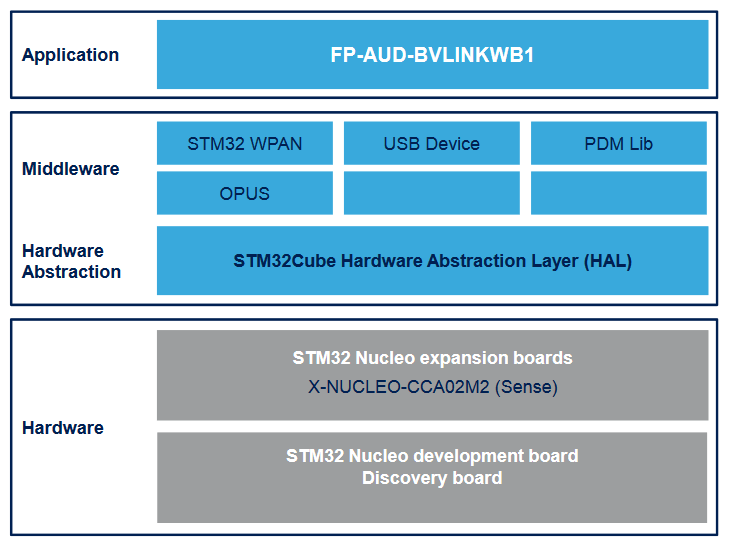
\includegraphics[width=\linewidth]{imgs/firmware_software_arch}
	\caption{Arhitektura softvera FP-AUD-BVLINKWB1}
	\label{fig:firmware_software_arch}
\end{figure}

Komponente za obradu funkcijskog paketa \textit{FP-AUD-BVLINKWB1} dizajnirane su za stvaranje bežične audio veze između modula odašiljača (Tx) i prijamnika (Rx), gdje mikrokontroler služi kao odašiljač, a računalo kao prijamnik. Cijeli lanac obrade zvuka počinje prijemom MEMS digitalnim mikrofonom i kulminira reprodukcijom zvuka na računalu.

BLE je konfiguriran za slanje paketa s maksimalnom veličinom od 150 bajtova. Ovisno o aplikaciji, kodirani bajtovi mogu biti iznad ovog praga, stoga komprimirani međuspremnik (engl. \textit{buffer}) mora biti podijeljen u više BLE paketa. Štoviše, veličina kodiranog međuspremnika može promijeniti svaki audio okvir i prijamnik mora znati njegovu duljinu da bi ga obnovio; za ovaj opseg implementiran je jednostavan protokol BLE prijenosa.

Na strani odašiljača, zvuk se dobiva digitalnim MEMS mikrofonom kao 1-bitni PDM signal i pretvara se pomoću filtra za pretvorbu PDM-u-PCM u 16-bitni PCM. Svaki put kad je audio okvir spreman, prenosi se u algoritam kompresije: veličina kodiranog međuspremnika koju vraća Opus koder može se značajno promijeniti u skladu s parametrima Opus kodera.

\begin{figure}[ht]
	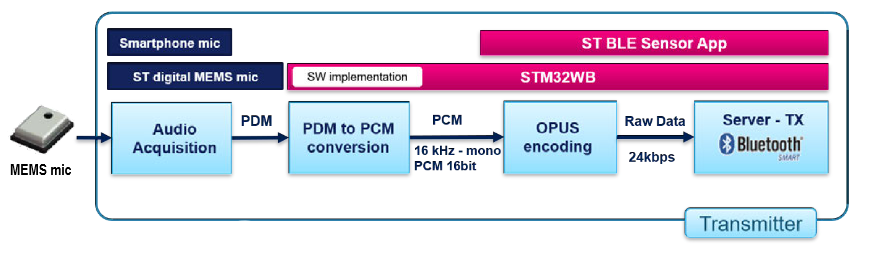
\includegraphics[width=\linewidth]{imgs/duplex_chain}
	\caption{Lanac obrade odašiljača u \textit{FP-AUD-BVLINKWB}}
	\label{fig:duplex_chain}
\end{figure}

\subsection{\textit{Middleware} za prijenos zvuka}

Budući da \textit{streaming} zvuka nije dio predefiniranog skupa profila mikrokontrolera, \textit{FP-AUD-BVLINKWB1} definira uslugu specifičnu za dobavljača pod nazivom \textit{BlueVoiceOPUS} koja je posrednik između korisničkog zvuka i  klijentskog uređaja. Ovisno o pokrenutoj aplikaciji, karakteristika se mijenja između audio ili glazbene karakteristike. Budući da \textit{streaming} glazbe nije implementiran u ovoj aplikaciji, opisane su samo audio karakteristike. 

Audio karakteristike sadrže sljedeće atribute:
\begin{itemize}
	\item \textit{Att1} - sadrži deklaraciju audio karakteristika,
	\begin{itemize}
		\item UUID: standardni 16-bitni UUID za karakterističnu deklaraciju
		\item Dozvole: R
		\item Vrijednost: svojstva za ovu karakteristiku su "\textit{notify only}", a UUID je za audio podatke
	\end{itemize}
	\item \textit{Att2} - sadrži audio podatke,
	\begin{itemize}
		\item UUID: isti UUID u zadnjih 16 bajtova vrijednosti atributa definicije karakteristike
		\item Dozvole: nema
		\item Vrijednost: stvarni audio sadržaj
	\end{itemize}
	\item \textit{Att3} - sadrži konfiguraciju karakteristika klijenta.
	\begin{itemize}
		\item UUID: standardni 16-bitni UUID za karakterističnu konfiguraciju klijenta
		\item Dozvole: R/W
		\item Vrijednost: prvi bit označava omogućenost obavijesti (0 ili 1), drugi bit omogućenost indikacija
	\end{itemize}
\end{itemize}

Usluga \textit{BlueVoiceOPUS} može implementirati odašiljač, prijamnik ili oboje u slučaju \textit{full-duplex} komunikacije. Za ovu aplikaciju potrebno je implementirati odašiljač odnosno transmiter.
Za prijenos zvuka, usluga i karakteristike moraju se kreirati pozivanjem \lstinline|BVOPUS_STM_Init()|, što uključuje funkcije \lstinline|BluevoiceOPUS_AddService()| i \lstinline|BluevoiceOPUS_AddChar()|; UUID-ovi su definirani u datoteci \lstinline|bvopus_service_stm.c|.

Karakteristike se mogu dodati već postojećoj usluzi pozivanjem \lstinline|BluevoiceOPUS_AddChar()| i prosljeđivanjem oznake te određene usluge kao parametra. Ako funkcija vrati \lstinline|BV_OPUS_SUCCESS|, BLE profil je ispravno kreiran.

Također, potrebno je konfigurirati Opus koder. U skladu sa traženim funkcijama, koder se može kreirati ispunjavanjem relevantne strukture \lstinline|OPUS_IF_ENC_ConfigTypeDef|.

Koder se može inicijalizirati pozivom \lstinline|BVOPUS_CodecEncInit(&EncConfigOpus)|. Ako funkcija vrati \lstinline|BV_OPUS_SUCCESS|, \textit{BlueVoiceOPUS} profil ispravno je konfiguriran. Ako vrati \lstinline|BV_OPUS_INVALID_PARAM|, neki od parametara nisu ispravni. Ovisno o odabranim parametrima, inicijalizacijska funkcija dodjeljuje količinu memorije koju relevantni API vraća interno. 

Pri inicijalizaciji podržani su sljedeći parametri:
\begin{itemize}
	\item \textit{application}: \lstinline|OPUS_APPLICATION_VOIP, OPUS_APPLICATION_AUDIO, OPUS_APPLICATION_RESTRICTED_LOWDELAY|,
	\item \textit{bitrate} [bps]: od 6000 do 510000,
	\item \textit{channels}: od 1 do 255,
	\item \textit{complexity}: od 0 do 10,
	\item \textit{ms\_frame} [ms]: 2.5, 5, 10, 20, 40, 60,
	\item \textit{sample\_freq} [Hz]: 8000, 12000, 16000, 24000, 48000.
\end{itemize}

\begin{lstlisting}[caption={Parametri za Opus koder}, language=c]
	EncConfigOpus.application = OPUS_APPLICATION_VOIP;
	/* bps */
	EncConfigOpus.bitrate = 24000; 
	/* 1 channel, mono*/
	EncConfigOpus.channels = AUDIO_CHANNELS_IN; 
	EncConfigOpus.complexity = 0;
	/* 20 ms */
	EncConfigOpus.ms_frame = AUDIO_IN_MS; 
	/* 16000 Hz */
	EncConfigOpus.sample_freq = AUDIO_IN_SAMPLING_FREQUENCY; 
\end{lstlisting}

Nakon postavljanja veze, modul koji je otkrio \textit{BlueVoiceOPUS} profil drugog modula mora omogućiti kontrolnu obavijest pozivanjem API-ja \lstinline|BluevoiceOPUS_EnableCtrl_Notif(void)|. Kontrolna se obavijest zatim koristi za zahtjev za pokretanje i zaustavljanje prijenosa.

Za početak audio prijenosa, modul odašiljača mora zatražiti od prijamnika da omogući njegovu audio obavijest pozivom \lstinline|BluevoiceOPUS_SendEnableNotifReq()|. Ovaj API šalje obavijest putem kontrolne karakteristike koja sadrži dva bajta (\lstinline|{BV_OPUS_CONTROL, BV_OPUS_ENABLE_NOTIF_REQ}|). Čim čvor primi zahtjev može omogućiti audio obavijest podnositelju zahtjeva pozivom funkcije \lstinline|BluevoiceOPUS_EnableAudio_Notif(void)|. Ako je obavijest ispravno omogućena, modul može započeti prijenos zvuka.

\textit{BlueVoiceOPUS} profil na ulaz prihvaća količinu PCM uzoraka jednaku veličini audio okvira postavljenoj tijekom Opus konfiguracije. Svaki put kada je audio okvir spreman, treba pozvati API \lstinline|BluevoiceOPUS_SendAudioData()| i on automatski sažima, fragmentira i šalje pakete audio podataka.

Za svaku primljenu zvučnu obavijest potrebno je pozvati \lstinline|BluevoiceOPUS_ParseData()| i provjeriti vraćeni status. U slučaju uspjeha, parametar \lstinline|pcm_samples| pokazuje je li spreman kompletan audio okvir.

Prema zadanim postavkama, Opus koder je konfiguriran s promjenjivom brzinom prijenosa: svaki kodirani okvir ima  duljinu prilagođenu brzini prijenosa postavljenoj tijekom faze inicijalizacije. Maksimalna veličina BLE paketa postavljena je na 150 bajtova, a broj BLE paketa može varirati među različitim audio okvirima ili ovisno o konfiguraciji Opusa.

Protokol prijenosa \textit{BlueVoiceOPUS} modula pokazuje kada kodirani podaci počinju i završavaju tako da prijamnik može ponovno izgraditi komprimirani međuspremnik i dekodirati ga: jedan bajt se dodaje kao prvi bajt svakog BLE paketa, preostalih 19 bajtova ili više, ovisno o odabranom MTU, popunjeni su podacima kodiranim Opusom.

Sljedeće vrijednosti mogu biti bajt zaglavlja:
\begin{itemize}
	\item \lstinline|BV_OPUS_TP_START_PACKET = 0x00|
	\item \lstinline|BV_OPUS_TP_START_END_PACKET = 0x20|
	\item \lstinline|BV_OPUS_TP_MIDDLE_PACKET = 0x40|
	\item \lstinline|BV_OPUS_TP_END_PACKET = 0x80|
\end{itemize}

Protokol prijenosa u potpunosti je obrađen u \textit{BlueVoiceOPUS} usluzi.
\subsection{Opus}
Opus je otvoren i svestran audio kodek koji se može koristiti za različite vrste aplikacija kao što su \textit{streaming} govora i glazbe ili komprimirana pohrana zvuka. Skalabilnost, od uskopojasnog govora niske brzine prijenosa pri 6 kbit/s do stereo glazbe pri 510 kbit/s niske složenosti, čini ga pogodnim za širok raspon interaktivnih aplikacija.

Sastoji se od dva sloja: jedan se temelji na linearnom predviđanju (LP), a drugi se temelji na modificiranoj diskretnoj kosinusnoj transformaciji (MDCT). Opus kombinira rezultate s gubitcima i bez gubitaka. Primjerice, u govornim aplikacijama, LP tehnike poput CELP-a (engl. \textit{Code-excited linear prediction}) učinkovitije kodiraju niske frekvencije nego u tehnikama transformacijske domene kao što je MDCT.

Opus kodek se sastoji od SILK i CELT tehnologija kodiranja. Prvi koristi model temeljen na predviđanju (LPC), dok je drugi u potpunosti modeliran na MDCT transformaciji. Ova svestranost omogućuje Opusu rad u tri načina rada (SILK, CELT ili hibridni način) i osigurava višestruke konfiguracije za različite aplikacije.

\section{Programska potpora za računalo}

Glavna zadaća aplikacije na računalu je primiti audio signal Bluetoothom, prikladno ga obraditi te izravno reproducirati i pohraniti. Za računalnu programsku potporu odabrana je \textit{BlueST-SDK} biblioteka koji omogućuje jednostavan pristup podacima koje izvozi BLE uređaj s implementiranim BlueST protokolom. Protokol BlueST lako je proširiv za podršku korisnički definiranih podataka. On već definira različite podatke koji dolaze iz različitih senzora kao što su inercijski senzori, senzori okoliša, informacije o bateriji, te DC i motori. Također implementira serijsku konzolu preko Bluetootha koja omogućuje funkcionalnost \textit{stdint}/\textit{stdout}/\textit{stderr} i definira konfiguracijski servis za kontrolu postavki povezanih ploča. 

Korištenjem zajedničkog modela programiranja za podržane platforme, \textit{BlueST-SDK} olakšava razvoj aplikacija na Android, iOS i Linux (s instaliranim Python) sustavima i uključuje primjere aplikacija koji demonstriraju korištenje SDK. Python izdanje \textit{BlueST-SDK} biblioteke koristi \textit{bluepy} Python biblioteku dostupnu na Linuxu za povezivanje s BLE uređajima.

\begin{figure}[ht]
	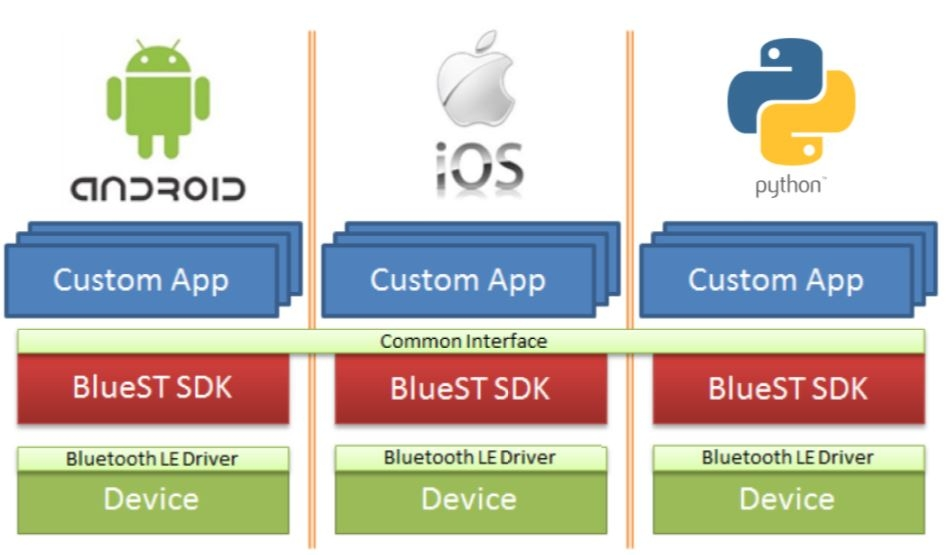
\includegraphics[width=\linewidth]{imgs/bluest_stack}
	\caption{Arhitektura aplikacije s \textit{BlueST-SDK} modulom}
	\label{fig:bluest_stack}
\end{figure}


Za razvoj aplikacije odabran je programski jezik Python na operacijskom sustavu Linux, koji nudi mnogobrojne biblioteke za snimanje i obradu zvuka. 


\begin{figure}[ht]
	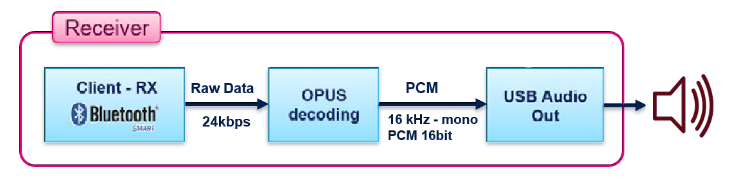
\includegraphics[width=\linewidth]{imgs/duplex_chain_2}
	\caption{Lanac obrade prijamnika u aplikaciji}
	\label{fig:duplex_chain_2}
\end{figure}